\begin{figure}[t]
\centering
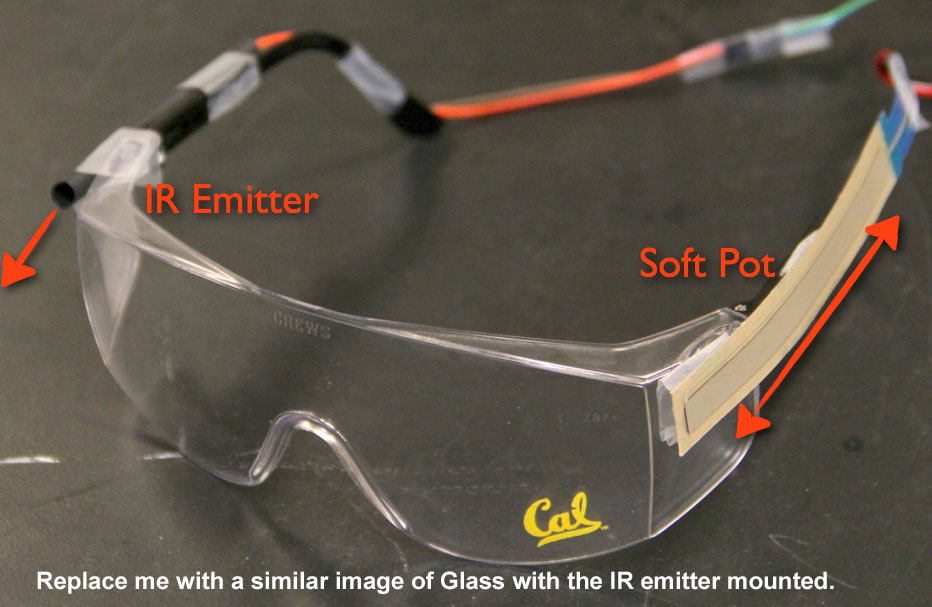
\includegraphics[width=1.0\columnwidth]{figures/glass-with-ir}
\caption{Our augmented Glass prototype has a frame-mounted infrared emitter.}
\label{fig:glass}
\end{figure}
\begin{figure}[t]
\centering
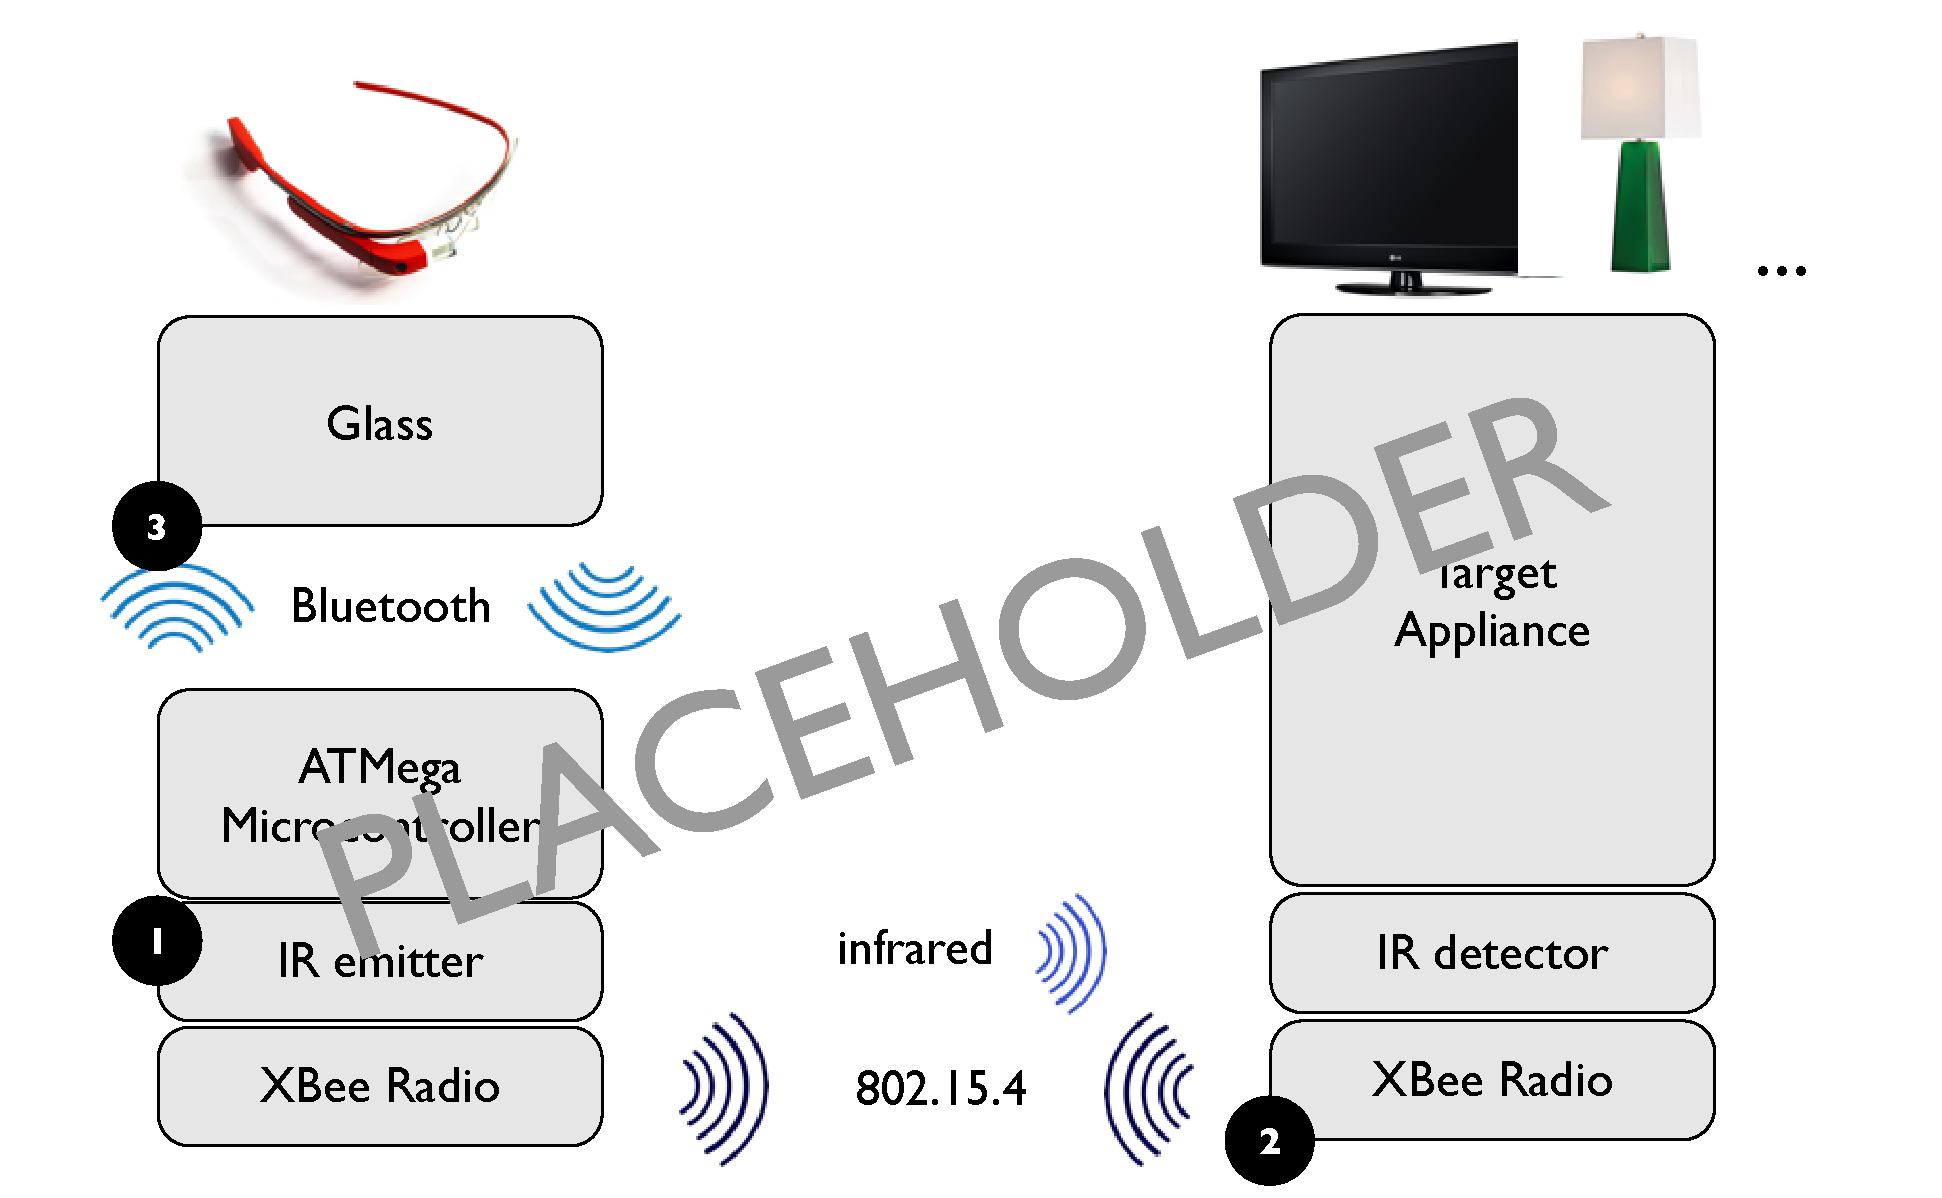
\includegraphics[width=1.0\columnwidth]{figures/architecture}
\caption{System architecture.}
\label{fig:architecture}
\end{figure}

\section{Hardware Device}

Our prototype consists of a Google Glass Explorer Edition head-worn computing device, augmented with an infrared emitter that is mounted on the frame, pointing out in the direction of the wearer's view (Figure~\ref{fig:glass}). The IR emitter LED is mounted in an opaque hollow tube, that restricts the outgoing angle of illumination. 

Glass communicates a device id over the IR channel analogous to Patel's approach~\cite{patel_2-way_2003}. Target appliances have IR receivers and offer immediate visual feedback by toggling an LED whenever a valid id is received.

When users confirm that, further communication switches over to a ZigBee wireless network so that line of sight to the target is no longer needed.

In our prototype, Glass communicates over Bluetooth to an additional microcontroller PCB the user has to wear (Atmel ATMega256). This board marshals XBee to Bluetooth messages in both directions and also controls the IR LED mounted on the Glass frame (Figure~\ref{fig:architecture}). This architecture was mostly chosen for reasons of expediency. We selected XBee 802.15.4 radios to avoid the latency associated with connecting and disconnecting to Bluetooth devices \bjoern{Is this true or not?} Future head-mounted devices could clearly integrate IR emitters; the choice of local wireless technology could also change. In particular, one could substitute WiFi modules. 

\subsection{Device Characterization}
We determined the usable range and accuracy empirically with one IR emitter and two IR receivers. The IR emitter constantly sent out an id signal. The receivers that correctly received the signal turn their LED on for 300 ms.

We placed all three devices at the same height with clear line of sight. The IR emitter is first places 2 feet away from the receivers. The receivers were moved sideways apart from each other until they could no longer receive stable signals. We then recorded the distance of the two receivers for the calculation of coverage angles. The steps are repeated for IR emitters in different distances (as shown in Table~\ref{table:measurements}). We then repeated measurements with the emitter  placed at various depths in the tube (see Figure~\ref{fig:coverage}). 

In summary, \bjoern{describe what the measured results mean in practice.}



\begin{figure}[t]
\centering
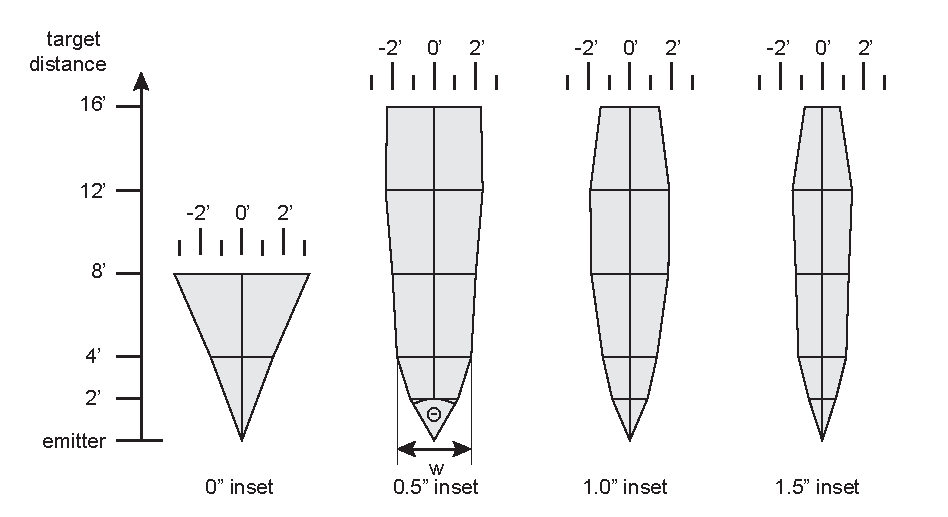
\includegraphics[width=1.0\columnwidth]{figures/glass-ir-coverage}
\caption{Our augmented Glass prototype has a frame-mounted infrared emitter.}
\label{fig:coverage}
\end{figure}

\begin{table}
    \begin{tabular}{l|lllll}
    distance/ depth & \ft2       & \ft4       & \ft8   & \ft{12}  & \ft{16}  \\ \hline
    \inch{0}                     & $74\degree$ & $78\degree$ & N/A  & N/A  & N/A  \\
  \inch{0.5}                   & $60\degree$ & $48\degree$     & $28\degree$ & $22\degree$ & $16\degree$ \\
    \inch{1.0}                     & $46\degree$     & $36\degree$     & $26\degree$ & $18\degree$ & $10\degree$ \\
    \inch{1.5}                   & $36\degree$     & $32\degree$     & $18\degree$ & $14\degree$ & $6\degree$  \\
    \end{tabular}
    \caption{Measured IR coverage angles $\Theta$ at different target distances and different depths of IR emitter inside shielding tube.}
    \label{table:measurements}
    
\end{table}